% This is an example on how to use the chalmers-thesis document class.
% Document should be compiled with pdflatex or lualatex
% If you find something odd, wrong or lacking, you can email me at; Mikael Öhman <mikael.ohman@chalmers.se>
% This file has been distributed through: http://www.github.com/Micket/chalmers

% These manuals are a *must* read. They are all full of good examples;
% amsldoc   - http://mirror.ctan.org/macros/latex/required/amslatex/math/amsldoc.pdf
% mathtools - http://mirror.ctan.org/macros/latex/contrib/mh/mathtools.pdf
% biblatex  - http://mirror.ctan.org/macros/latex/contrib/biblatex/doc/biblatex.pdf
% booktabs  - http://mirror.ctan.org/macros/latex/contrib/booktabs/booktabs.pdf
% http://www.ctan.org/tex-archive/help/Catalogue/bytopic.html
% http://en.wikibooks.org/wiki/LaTeX/

\RequirePackage[l2tabu,orthodox]{nag} % This package helps prevent you from doing things wrong.

% change doctorate to licentiate if necessary
\documentclass[licentiate,nocover,g5paper,11pt]{gu-thesis}
% All options are; doctorate, licentiate, masters, bachelors, nocover, draft, g5paper,
% and everything the standard report class support.
%\usepackage{ifluatex} % Automatic check for luatex.
%\ifluatex
% \usepackage{fontspec}
%\else
\usepackage[utf8]{inputenc} % File encoding, you should try to stick to utf8.
%\fi
\usepackage{microtype} % Magically improves typesetting for pdflatex
\usepackage{subfiles} % Convenient use of subfiles in documents. Using \subfile is optional. See README
\usepackage{hyperref} % Required for in document links and document metadata.
\usepackage[swedish, english]{babel}

\newcommand{\todo}[1]{{\color{red}#1}}
%\usepackage[draft]{graphicx}
% More or less required packages
%\usepackage{csquotes} % Needed for biblatex
%\usepackage[firstinits=true, style=alphabetic, backend=biber]{biblatex} % Modern bibliography facilities (you may change style to numeric). change to old bibtex if you insist on using that.
 
\usepackage[square,numbers,sort&compress]{natbib}
\usepackage{bibentry}
\bibliographystyle{jfm}


\usepackage{mathtools} % All your math related needs
\usepackage{tikz} % Draw figures, required for cover page
%\usepackage{subfigure} % Subfloats
\usepackage[list=off]{caption}
\captionsetup{singlelinecheck=off}
\usepackage{subcaption}
% Read the manuals for the respective package to see the usage;
\usepackage{pdfpages} % For included other pdf files (like articles).
%\usepackage{thmtools} % For theorems.
%\usepackage{algorithms} % For algorithms.
\usepackage{listings} % For source code.
\usepackage{booktabs} % High quality tables.
%\usepackage{siunitx} % For all your numerical values and units. 
%\usepackage{pgfplots} % Make plots directly in latex. Also tables. Excellent package.
%\usepackage{contmech} % Custom package for typesetting in continuum mechanics for applied mechanics.
%\usepackage{yourcustomcommands} % Put your custom commands in a file 'yourcustomcommands.sty' and load it like this.

% JONAS
\usepackage{afterpage}

\usepackage[bbgreekl]{mathbbol}
%\usepackage{amssymb}


\newcommand{\ve}[1]{\ensuremath{\mbox{\boldmath$#1$}}}
\newcommand{\ma}[1]{\ensuremath{\mathbb{#1}}}
\newcommand{\te}[1]{\ensuremath{\mathscr{#1}}}

\newcommand{\CC}[2]{\ensuremath{{\cal C}{{#1}_;}{#2}}}
\newcommand{\DD}{\ensuremath{{\cal D}}}
\newcommand{\ku}{\ensuremath{\mbox{Ku}}}
\newcommand{\st}{\ensuremath{\mbox{St}}}
\newcommand{\steff}{\ensuremath{\widetilde \st}}
\newcommand{\pe}{\ensuremath{\mbox{Pe}}}
\newcommand{\per}{\ensuremath{\mbox{Pe}_{\mathrm r}}}
\newcommand{\re}{\ensuremath{\mbox{Re}}}
\newcommand{\rep}{\ensuremath{\mbox{Re}_{\mathrm p}}}
\newcommand{\tr}{\ensuremath{\mbox{Tr}}}
\newcommand{\sign}{\ensuremath{\mbox{sign}}}
\newcommand\transpose{^{\mathrm T}}
\newcommand{\diff}[2]{\frac{\rd #1}{\rd #2}}
\newcommand{\pdiff}[2]{\frac{\partial #1}{\partial #2}}
\newcommand{\ii}{{\rm i}}

\newcommand{\spma}[1]{#1\ve n - \ve n(\ve n\transpose #1\ve n)}
\newcommand{\venn}{\ve n \ve n\transpose}
\newcommand{\maid}{\ma I}

\newcommand{\Ordo}{\ensuremath{O}}
\newcommand{\ordo}{\ensuremath{o}}

\newcommand{\evalat}[1]{\,\bigg|_{#1}}
\newcommand{\rd}{\ensuremath{\mathrm{d}}}


\newcommand\nn{\nonumber}

\newcommand{\eqnlab}[1]{\label{eqn:#1}}
\newcommand{\figlab}[1]{\label{fig:#1}}
\newcommand{\tablab}[1]{\label{tab:#1}}
\newcommand{\eqnref}[1]{(\ref{eqn:#1})}
\newcommand{\figref}[1]{\ref{fig:#1}}
\newcommand{\tabref}[1]{\ref{tab:#1}}
\newcommand{\Eqnref}[1]{Eq.~(\ref{eqn:#1})}
\newcommand{\Figref}[1]{Fig.~\ref{fig:#1}}
\newcommand{\Tabref}[1]{Table~\ref{tab:#1}}
\newcommand{\Eqsref}[1]{Eqs.~(\ref{eqn:#1})}
\newcommand{\Figsref}[1]{Figs.~\ref{fig:#1}}
\newcommand{\Tabsref}[1]{Tables~\ref{tab:#1}}

\newcommand{\applab}[1]{\label{app:#1}}
\newcommand{\chlab}[1]{\label{ch:#1}}
\newcommand{\seclab}[1]{\label{sec:#1}}
\newcommand{\sseclab}[1]{\label{ssec:#1}}
\newcommand{\appref}[1]{\ref{app:#1}}
\newcommand{\chref}[1]{\ref{ch:#1}}
\newcommand{\secref}[1]{\ref{sec:#1}}
\newcommand{\ssecref}[1]{\ref{ssec:#1}}
\newcommand{\Appref}[1]{Appendix~\ref{app:#1}}
\newcommand{\Chref}[1]{Chapter~\ref{ch:#1}}
\newcommand{\Secref}[1]{Section~\ref{sec:#1}}
\newcommand{\Ssecref}[1]{Subsec.~\ref{ssec:#1}}
\newcommand{\Chsref}[1]{Chapter~\ref{ch:#1}}
\newcommand{\Secsref}[1]{Sections.~\ref{sec:#1}}
\newcommand{\Ssecsref}[1]{Subsecs.~\ref{ssec:#1}}
\newcommand{\obs}[1]{{\color{red}#1}}
\newcommand{\Reys}{\ensuremath{\textrm{Re}_s}}	
%\newcommand{\Ylm}[2]{Y_#1^#2(\ve n)}
\newcommand{\Ylm}[2]{|#1,#2\rangle}
\newcommand{\cross}{\times}
\newcommand{\dd}{\colon}
\newcommand{\lc}{\varepsilon}
\newcommand{\proofheader}[1]{\emph{#1}}
\usepackage{wrapfig}
\usepackage{units}
\usepackage{url}
\usepackage{upgreek}
\usepackage{lpic}
\usepackage{csquotes}
\setquotestyle{swedish}
% END JONAS

\urlstyle{same}

%\newcommand{\paperAaddress}{http://dx.doi.org/10.1007/s00707-013-0924-0}
% FONT

% 1
%\usepackage[sc]{mathpazo}
%\usepackage{tgpagella}
%\usepackage[T1]{fontenc}

%2
\usepackage[adobe-utopia]{mathdesign}
\usepackage[T1]{fontenc}


% fancyhdr
\usepackage{overpic}
\usepackage{fancyhdr}
\usepackage{flipbook}



\fancypagestyle{fb}
{%
\fancyhf{}%
\renewcommand{\headrulewidth}{0pt}
\rfoot[]{%
  \setlength\unitlength{1cm}%
  \begin{picture}(0,0)%
    \put(0.0,-2){%
      \fbImageF{./figs/plotting/flipbook/output/symm/}{png}{width=20mm}%
    }%
  \end{picture}%
}
\lfoot[%
  \setlength\unitlength{1cm}
  \begin{picture}(0,0)
    \put(-2.5,-2){
      \fbImageF{./figs/plotting/flipbook/output/triax/}{png}{width=20mm}
    }
  \end{picture}
]{}
}


\pagestyle{fancy}
\setlength{\headheight}{15pt}

\renewcommand{\partmark}[1]{ \markboth{#1}{} }
\renewcommand{\chaptermark}[1]{ \markboth{#1}{} }
\renewcommand{\sectionmark}[1]{ \markright{#1}{} }

\fancyhf{}
\fancyhead[LE,RO]{\textsc {\thepage}}
\fancyhead[RE]{\textsc{ \nouppercase{\leftmark}} }
\fancyhead[LO]{\textsc{ \nouppercase{\rightmark}} }

\rfoot[]{%
  \setlength\unitlength{1cm}
  \begin{picture}(0,0)
    \put(0.0,-2){
      \fbImageF{./figs/plotting/flipbook/output/symm/}{png}{width=20mm}
    }
  \end{picture}
}
\lfoot[%
  \setlength\unitlength{1cm}
  \begin{picture}(0,0)
    \put(-2.5,-2){
      \fbImageF{./figs/plotting/flipbook/output/triax/}{png}{width=20mm}
    }
  \end{picture}
]{}


%\fancypagestyle{plain}{ %
%  \fancyhf{} % remove everything
%  \renewcommand{\headrulewidth}{0pt} % remove lines as well
%  \renewcommand{\footrulewidth}{0pt}
%}

%%%%


% User commands
\title{Angular dynamics of small particles in fluids}
%\subtitle{And Perhaps a Subtitle}
\author{Jonas Einarsson} % Not common with more than one author
\thesisin{Physics}
\department{Department of Physics}
%\division{Division of Solid Mechanics}
\reportno{2013:01}
\ISBN{TODO} % Only for doctorate
\copyrightyear{2015}

\opponent{
Title Name \\
Department \\
University \\
Country
}
\oppositiondate{When, and where}

% You should scale the figure according to textwidth and or paperheight.
%\coverfigure{\includegraphics[width=\textwidth,height=0.4\paperheight,keepaspectratio]{figures/ExampleCover}}
%\covercaption{Some explanation}

\firstabstract{%
This thesis concerns the angular motion of small particles suspended in fluid flows. A small particle experiences a hydrodynamic torque due to the local fluid velocity, and this torque leads to rotational motion. When inertial effects are negligible the torque on an ellipsoidal particle is given by
Jeffery's theory [\textsc{Jeffery, G. B.} \emph{Proc. R. Soc. Lond. A} \textbf{102},~161–179~(1922)].
In this thesis and the appended papers I describe three studies that all relate to this well-known result.

First, we derive an effective equation of motion for the orientation of a spheroid in a simple shear flow, valid for small values of the shear Reynolds number $\Reys=sa^2/\nu$, where $s$ is the shear rate, $a$ the particle size and $\nu$ the kinematic viscosity of the suspending fluid. In absence of inertia the equation of motion has infinitely many periodic solutions, the {\lq}Jeffery orbits{\rq}. We show how this degeneracy is lifted by the effects of inertia.

Second, we describe experimental observations of the orientational dynamics of asymmetric particles advected in a microchannel. We record several trajectories with each particle by resetting the initial condition with an optical trap. We find that the dynamics depend sensitively on both particle shape and initial conditions. This confirms earlier theoretical results, which are also described in this thesis.

Third, we discuss the angular dynamics of axisymmetric particles in turbulent and random flow. In these flows the statistical averages of the angular dynamical quantities depend crucially on the intricate correlations between the particle orientation, angular velocity, and the flow vorticity relative to the principal straining directions of the fluid flow. We illustrate this by direct numerical simulation, experimental measurements and statistical model calculations.

Finally, this thesis contains an introduction to the field aimed at new students, as well as an accessible popular science introduction to low Reynolds particle dynamics. 
}
%\secondabstract{swedish}{Text}
\keywords{}

%\preface{Text}
\acknowledgements{
Although written by my hand, this thesis is by no means conceived by me alone. I am most grateful for the enthusiastic guidance from my supervisor Bernhard Mehlig. It is a privilege to work with someone with the physical insight, unquenchable enthusiasm and sheer perseverance it takes to get things right.

Further, I am indebted to all our collaborators for their work. Fabien Candelier and Jean-R\'egis Angilella in France for teaching me fluid dynamics. Greg Voth and Evan Variano in the US for the wonderful experiments and discussions, and our experimental collegues in Dag Hanstorp's lab for hunting the Jeffery orbits with us.

I also want to thank my present and former collegues for the open scientific environment at the department. In particular I appreciate the company of my fellow students Kristian Gustafsson, Marina Rafajlovi\'c and Erik Werner (who all graduated before me), and I welcome our new students Johan Fries and Jan Meibohm to this group. An extra thank you to Erik and Jan who improved this thesis with their helpful comments. Any remaining mistakes are mine alone.

Finally, I am fortunate to have my wonderful family. Thank you Freja and Tora for giving meaning to it all $\heartsuit$.
}
%\paperwork{Text}

\printers{Kompendiet}

% You can add extra contents such as abbreviations and nomenclature using.
% Use \presectiontitle to render add titles to new sections.
% \extrafrontmatter{\presectiontitle{Nomenclature} Text} % Optional

% Other optional settings for biblatex;
% \DeclareFieldFormat[article]{title}{#1} % Removes quotes from article title
% \DeclareFieldFormat[article]{volume}{\mkbibbold{#1}} % Makes volume print in bold.
% \renewbibmacro{in:}{} % Removes the "In:" from the journals field.
% \DeclareFieldFormat[article]{pages}{#1} % Removes the pp. before pages.
% % Adds short journal entries;
% \renewbibmacro*{journal+issuetitle}{%
%   \usebibmacro{shortjournal}%
%   \setunit*{\addspace}%
%   \iffieldundef{series}{}{\newunit\printfield{series}\setunit{\addspace}}%
%   \usebibmacro{volume+number+eid}%
%   \setunit{\addspace}%
%   \usebibmacro{issue+date}%
%   \setunit{\addcolon\space}%
%   \usebibmacro{issue}%
%   \newunit}
% % End of optional citation modifications.

%\addbibresource{references.bib} % New command, use if available


\setlength{\topcolumn}{0.22\textwidth} % Column for "Thesis" page which might need adjustments if there is other publications.
\usepackage{enumitem}
\begin{document}

%% TITLE
\pagestyle{empty}
\pagenumbering{roman}
\setcounter{page}{-100} % for hyperref, odd right sides
~\newpage
\maketitlepage
\clearpage\makeprintinfopage
\cleardoublepage\makeabstractpage
\cleardoublepage\maketableofpaperspage



\cleardoublepage
\setcounter{tocdepth}{1}
\tableofcontents

\cleardoublepage\pagenumbering{arabic}
\pagestyle{fancy}
\part{Introduction}
\thispagestyle{fb}
\subfile{partI}
\clearpage\thispagestyle{fb}\cleardoublepage\thispagestyle{fb}
{
\null\vfill
\centering
\parbox{8cm}{%
  \raggedright{\large\itshape%
Men då mitt skarpsinne visade sig otillräckligt även för detta, slungade jag schackbrädet ut genom fönstret i huvudet på en gammal man med träben, för vilken döden endast var en välgärning, och kastade mig därefter ut i världsvimlet, föraktande mig själv.\par\bigskip
  }   
  \raggedleft\large{ur \emph{Spleen}, av Hjalmar Söderberg}\par%
}
\vfill\vfill
}



\newpage\thispagestyle{fb}\cleardoublepage
\part{My work}
\thispagestyle{fb}
\subfile{partII}
\clearpage\thispagestyle{fb}\cleardoublepage
\thispagestyle{fb}
{
\null\vfill
\centering
\parbox{8cm}{%
  \raggedright{\large\itshape%
Blåsten visslar i fönsterspringorna, och regnet porlar i takrännan, och nu är sagan slut. Den som icke har förstått den kan trösta sig med att det blir vackert väder imorgon.\par\bigskip
  }   
  \raggedleft\large{ur \emph{Duggregnet}, av Hjalmar Söderberg}\par%
}
\vfill\vfill
}
\newpage\thispagestyle{fb}\cleardoublepage
\thispagestyle{fb}\makeacknowledgementspage
\clearpage\thispagestyle{fb}\cleardoublepage
\pagestyle{fancy}
%\nocite{paperA,paperB,paperC,paperD,paperE,paperF,paperG}
\nobibliography*
\bibliography{references} % Legacy command
\clearpage\thispagestyle{fb}\cleardoublepage
\part*{Appendix} % Using the starred command avoids numbering.
\appendix
\thispagestyle{fb}
\subfile{app_triaxial_equations}

\clearpage\thispagestyle{fb}\cleardoublepage
\label{endpage}\part{Papers}
\pagestyle{fb}
\paper{Paper A}{%
{\sc Einarsson, J, Candelier, F, Lundell, F, Angilella, J.~R \& Mehlig, B}
  2015{\natexlab{{\em a\/}}} Effect of weak fluid inertia upon {J}effery orbits.
  {\em Physical Review E\/} {\bf 91}~(4), 041002.%
}{Open Access (CC BY 3.0) at \url{http://dx.doi.org/10.1103/PhysRevE.91.041002}}
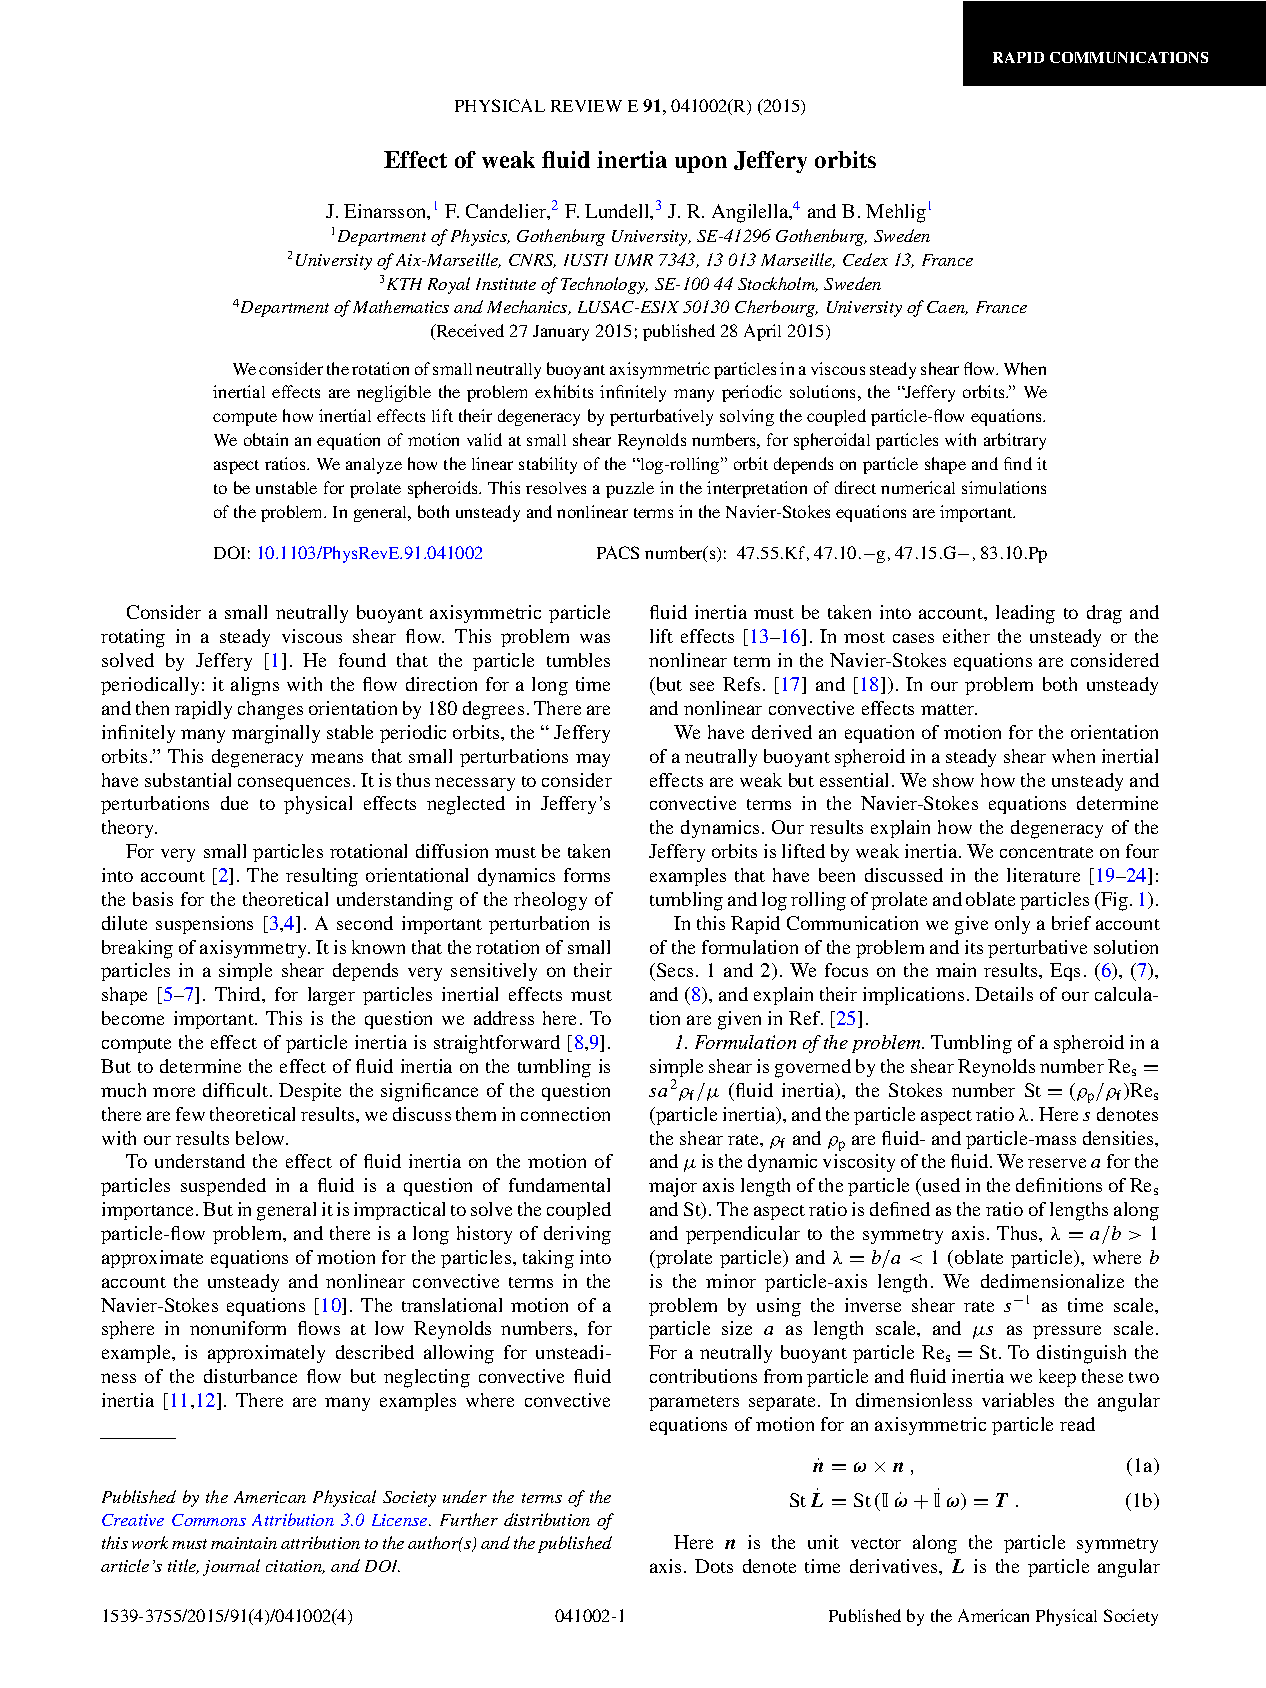
\includepdf[pages=-,width=\paperwidth,pagecommand={\thispagestyle{fb}}]{papers/A.pdf}

\paper{Paper B}{%
{\sc Candelier, F, Einarsson, J, Lundell, F, Mehlig, B \& Angilella, J.~R} 2015
  Role of inertia for the rotation of a nearly spherical particle in a general
  linear flow. {\em Physical Review E\/} {\bf 91}~(5), 053023.%
}{arXiv preprint available at \url{http://arxiv.org/abs/1505.02661}}
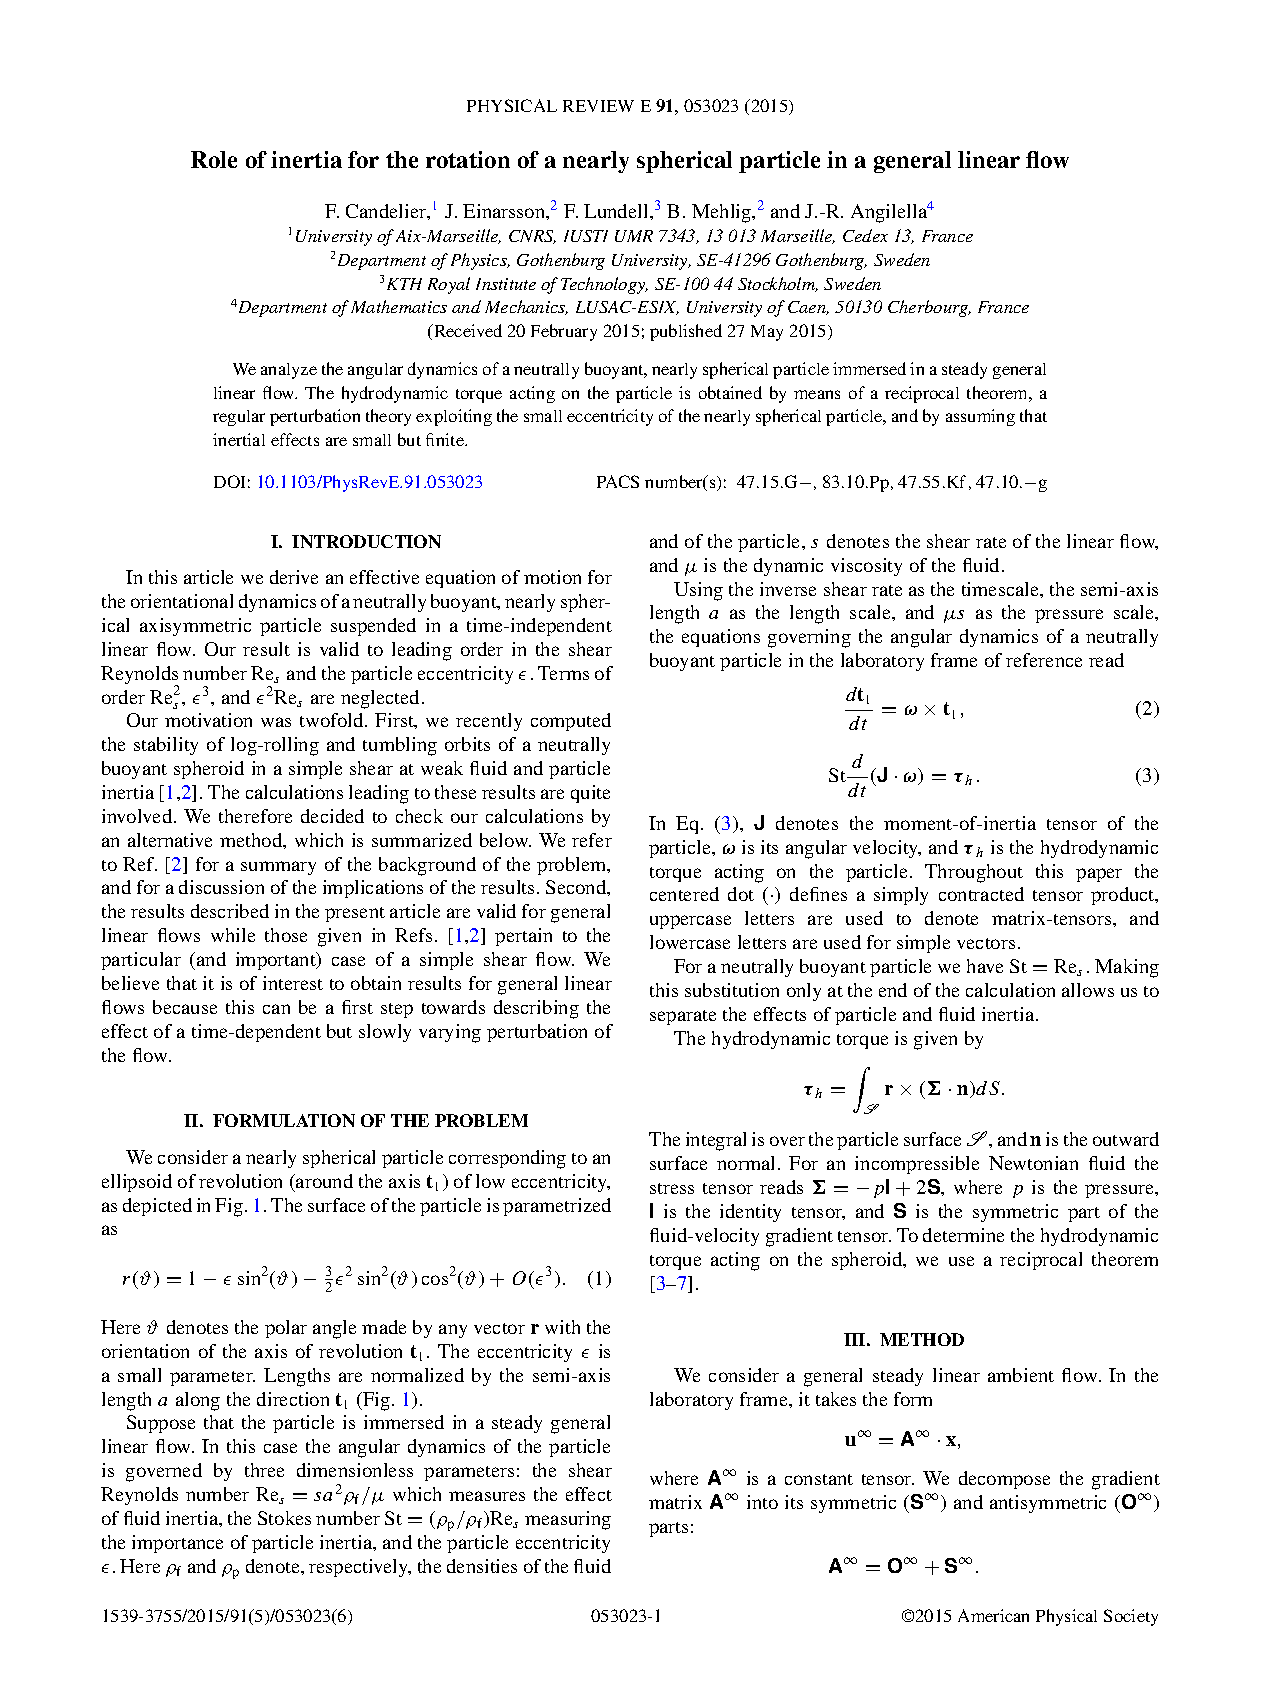
\includepdf[pages=-,width=\paperwidth,pagecommand={\thispagestyle{fb}}]{papers/B.pdf}
\includepdf[pages=3-,width=\paperwidth,pagecommand={\thispagestyle{fb}}]{papers/Bc.pdf}

\paper{Paper C}{%
{\sc Einarsson, J, Candelier, F, Lundell, F, Angilella, J.~R \& Mehlig, B}
  2015{\natexlab{{\em b\/}}} Rotation of a spheroid in a simple shear at small
  {R}eynolds number. {\em Physics of Fluids\/} {\bf 27}~(6),
  063301.%
}{Open Access (CC BY 3.0) at http://dx.doi.org/10.1063/1.4921543}

\includepdf[pages=2-,width=\paperwidth,pagecommand={\thispagestyle{fb}}]{papers/C.pdf}


\paper{Paper D}{%
{\sc Rosen T, Einarsson, J, Nordmark, A, Aidun, C. K, Lundell, F \& Mehlig, B} 2015
  Numerical analysis of the angular motion of a neutrally buoyant spheroid in shear flow at small Reynolds numbers. {\em Physical Review E (in review)\/}. arXiv \href{http://arxiv.org/abs/1508.04976}{1508.04976}. %
}{arXiv preprint available at \url{http://arxiv.org/abs/1508.04976}}
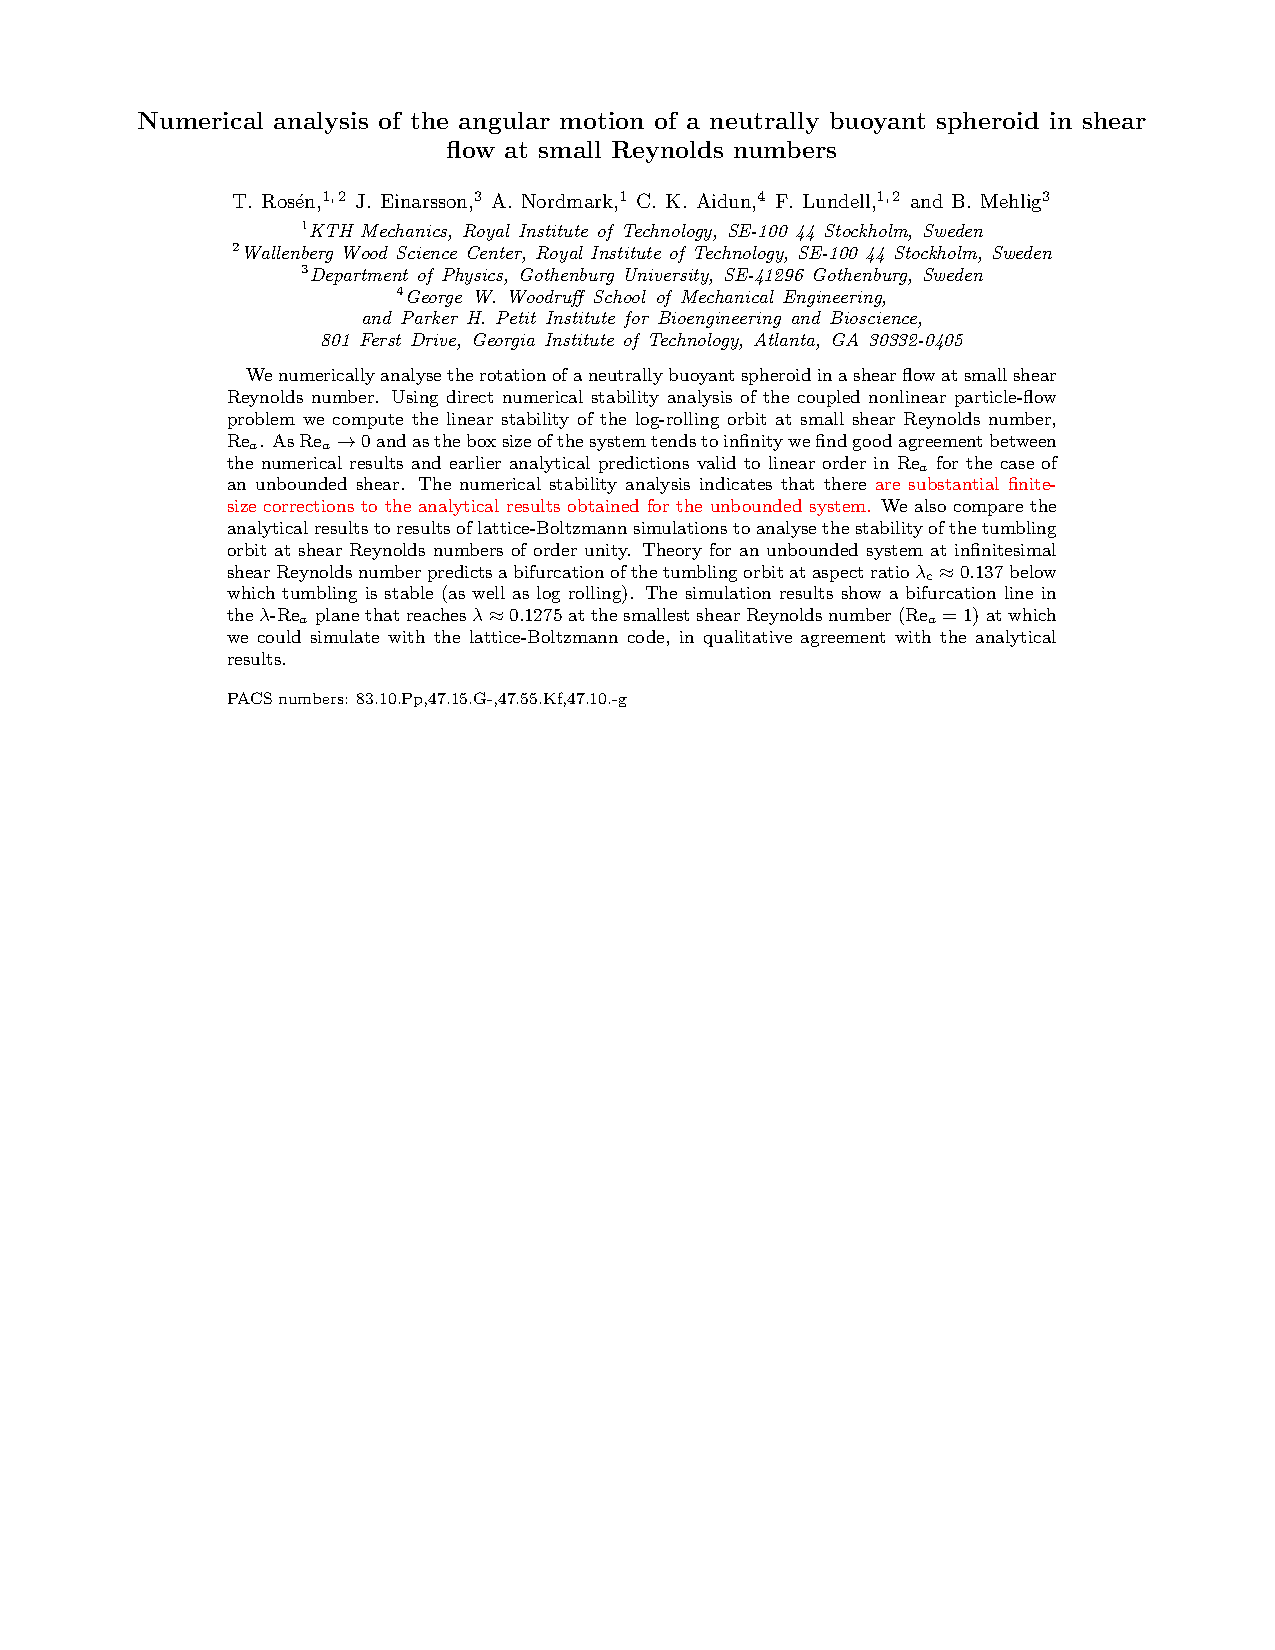
\includepdf[pages=-,width=\paperwidth,pagecommand={\thispagestyle{fb}}]{papers/D.pdf}


\paper{Paper E}{%
{\sc Einarsson, J, Mihiretie, B. M, Laas, A, Ankardal, S, Angilella, J. R, Hanstorp, D, \& Mehlig, B} 2015
  Tumbling of asymmetric microrods in a microchannel flow. {\em Physics of Fluids (in review)\/}. arXiv \href{http://arxiv.org/abs/1503.03023}{1503.03023}%
}{arXiv preprint available at \url{http://arxiv.org/abs/1503.03023}}
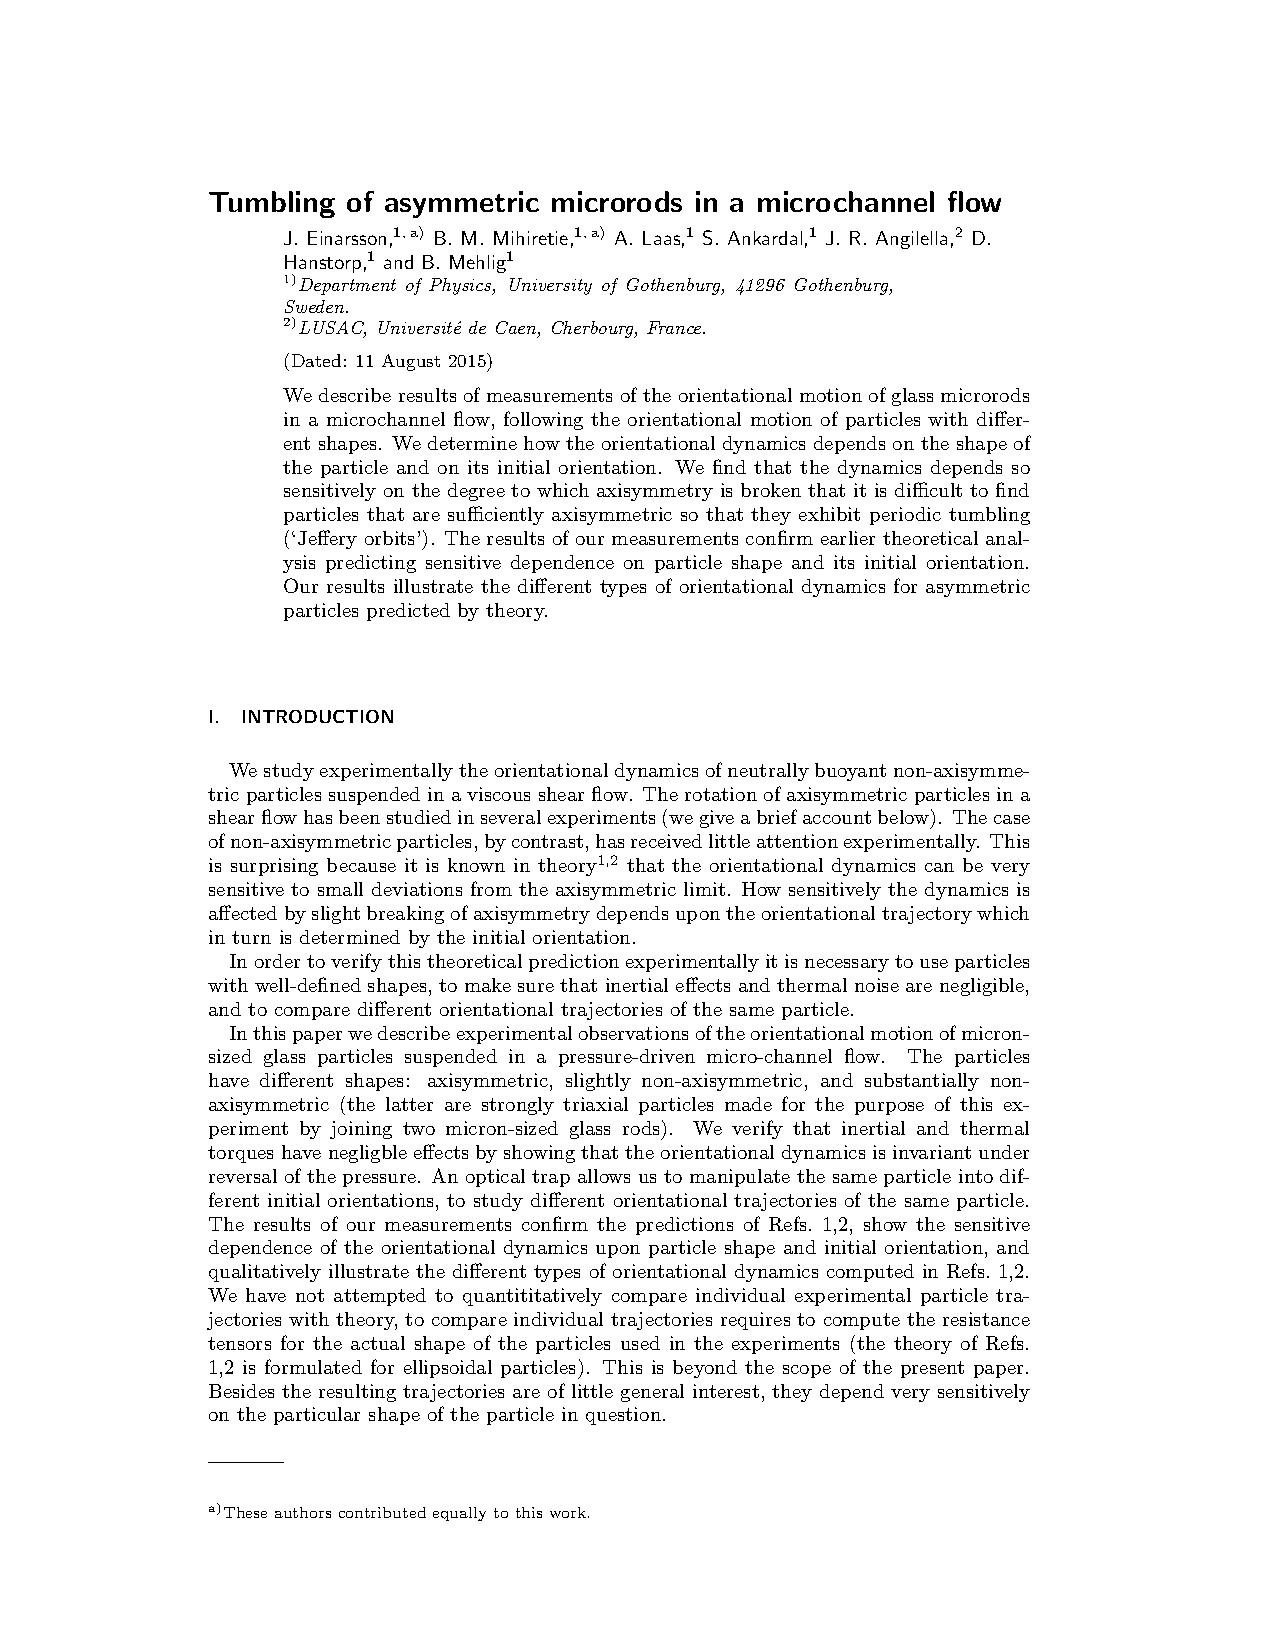
\includepdf[pages=-,width=\paperwidth,pagecommand={\thispagestyle{fb}}]{papers/E.pdf}
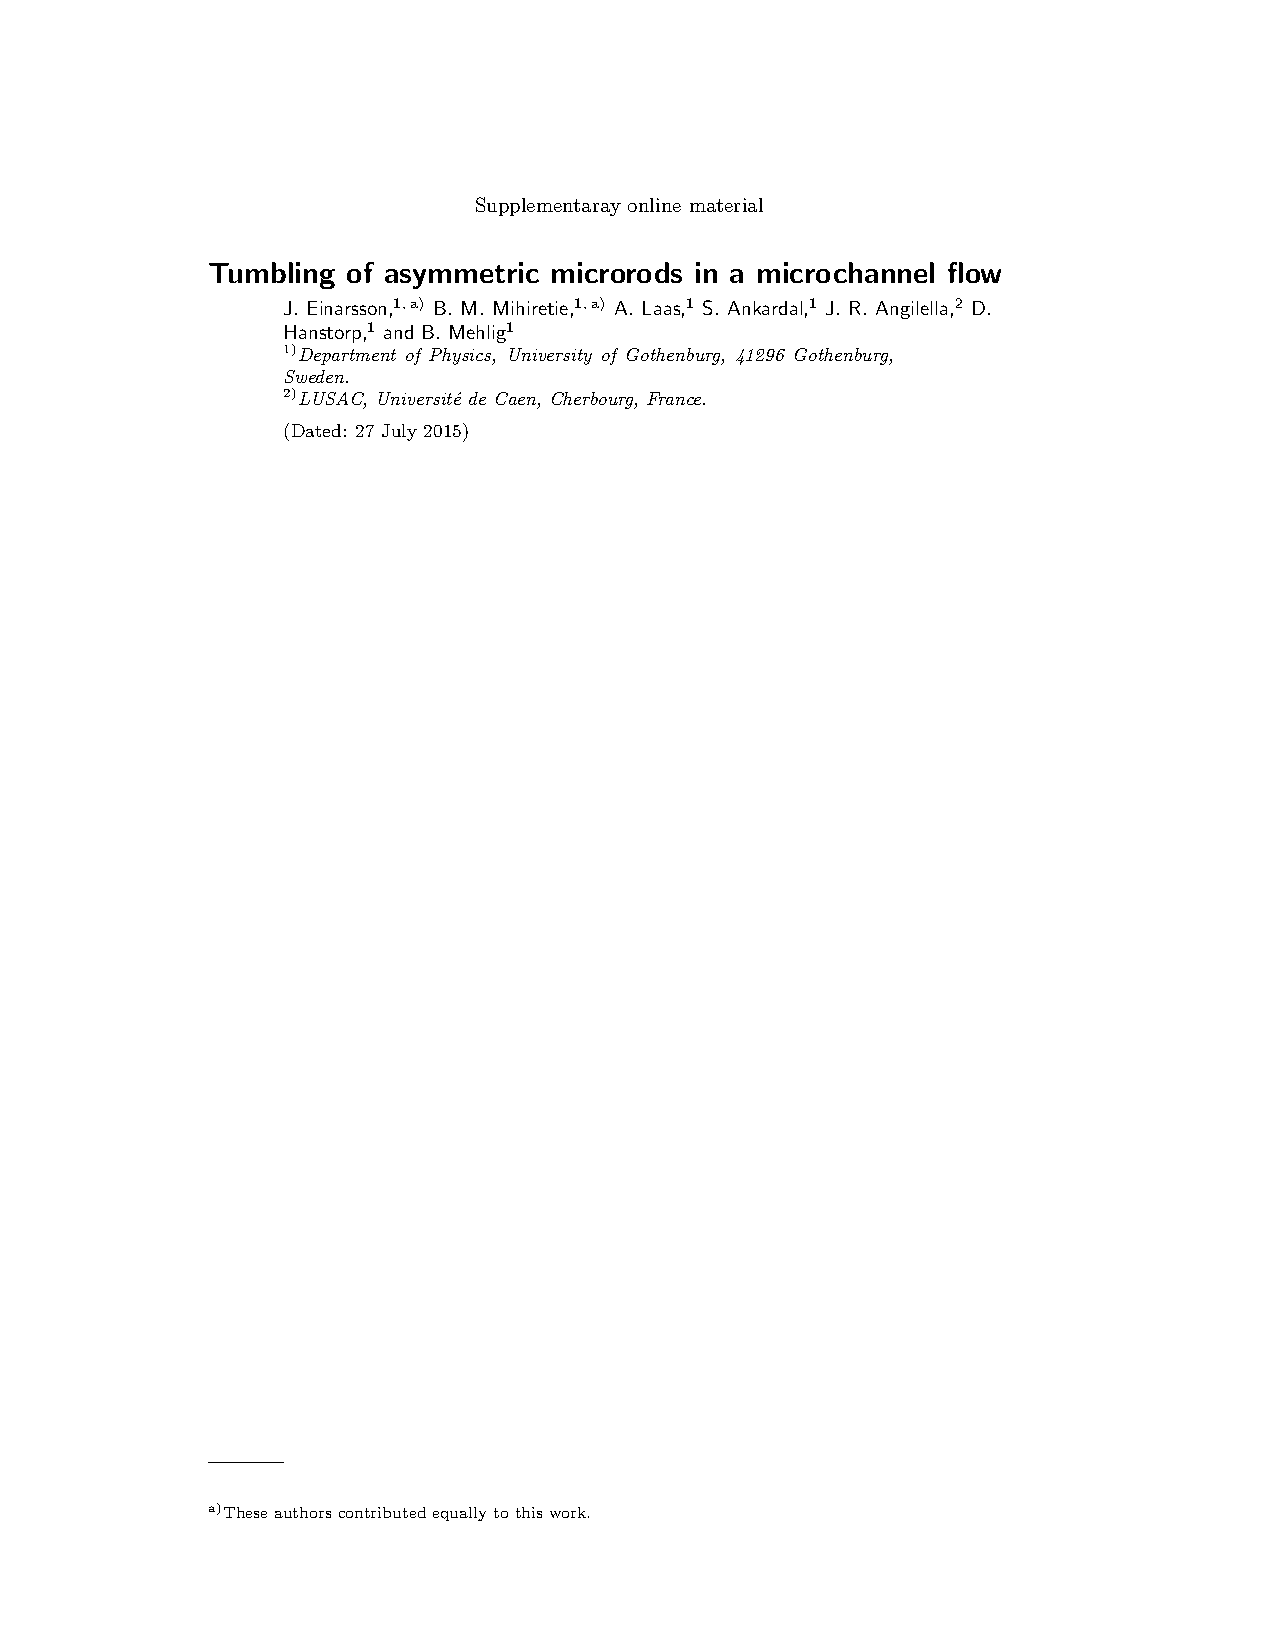
\includepdf[pages=-,width=\paperwidth,pagecommand={\thispagestyle{fb}}]{papers/Es.pdf}


\paper{Paper F}{%
{\sc Byron, M, Einarsson, J, Gustavsson, K, Voth, G, Mehlig, B \& Variano, E}
  2015 Shape-dependence of particle rotation in isotropic turbulence. {\em
  Physics of Fluids\/} {\bf 27}~(3), 035101.%
}{arXiv preprint available at \url{http://arxiv.org/abs/1412.3166}}
\includepdf[pages=2-,width=\paperwidth,pagecommand={\thispagestyle{fb}}]{papers/F.pdf}


\pagestyle{fb}
\cleardoublepage


\end{document}
 